\documentclass[10pt,a4paper]{article}
\usepackage[latin1]{inputenc}
\usepackage{amsmath}
\usepackage{amsfonts}
\usepackage{amssymb}
\usepackage{graphicx}
\usepackage{multicol}
\usepackage{changepage}
\usepackage{float}
\usepackage{cite}
\usepackage{url}
\usepackage{imakeidx}
\makeindex

\usepackage[left=2.50cm, right=2.50cm]{geometry}
\usepackage[spanish]{babel}

\author{Axel}
\title{Portada siempre practica}

\begin{document}
%encabezado 
\pagestyle{plain}{
\pagestyle{empty}
\changepage{3cm}{1cm}{-0.5cm}{-0.5cm}{}{-2cm}{}{}{}
\noindent

%sEGIUN EL formato de sus imagenes, deben encontrar una configuracion adeacuada para ustedes
{\small
\begin{tabular}{p{0.626\textwidth} p{0.50\textwidth} }

\includegraphics[scale=0.26]{uaem.jpg} &  
\includegraphics[scale=0.3]{ico.jpg}
\end{tabular}
}

%datos de la caratula
\begin{center}
\par\vspace{2cm} %Rspacoo dejado antes del encabezado
{
\Huge\textbf{
Universidad Aut\'onoma del Estado de M\'exico \\[1cm] Ingenier\'ia en Computaci\'on
}
}
\par\vspace{1.5cm}
{
\Large\textbf{ Materia: Algoritmos Gen\'eticos \\ Laboratorio 04
}
}
\par\vspace{1.5cm}
{
\large\textbf{Axel Valenzuela Ju\'arez \\Profesor: Dr. Asdr\'ubal	L\'opez	Chau \\ 14 de Marzo del 2020 } 
}

\par\vspace{1.5cm}

\end{center}
\clearpage

}

\printindex

\section{
Introducci\'on
}

\paragraph{
Los Algoritmos Gen\'eticos son m\'etodos adaptativos que pueden usarse para resolver problemas de b\'usqueda y optimizaci\'on. Est\'an basados en el proceso gen\'etico de los organismos vivos.
}
\paragraph{
Los Algoritmos Gen\'eticos son capaces de ir creando soluciones para problemas del mundo real.
}
\paragraph{
El poder de los Algoritmos Gen\'eticos proviene del hecho de que se trata de una t\'ecnica robusta,
y pueden tratar con \'exito una gran variedad de problemas provenientes de diferentes \'areas, incluyendo aquellos en los que otros m\'etodos encuentran dificultades. Si bien no se garantiza que el Algoritmo Gen\'etico encuentre la soluci\'on optima del problema, existe evidencia emp\'irica de que se encuentran soluciones de un nivel aceptable, en un tiempo competitivo con el resto de los algoritmos de optimizaci\'on combinatoria. En el caso de que existan t\'ecnicas especializadas para resolver un determinado problema, lo m\'as probable es que superen al Algoritmo Gen\'etico, tanto en rapidez como en eficacia.
}
\paragraph{
 El gran campo de aplicaci\'on de los Algoritmos Gen\'eticos se relaciona con aquellos problemas para los cuales no existen t\'ecnicas especializadas. Incluso en el caso en que dichas t\'ecnicas existan, y funcionen bien, pueden efectuarse mejoras de estas hibrid\'andolas con los Algoritmos Gen\'eticos.
}
\newpage
\section{Desarrollo}
\paragraph{
La implementaci\'on del primer algoritmo gen\'etico del curso se realizo de manera diferente en este caso, ya que se nos fue presentado el algoritmo de un fragmento de libro el cual deb\'iamos leer y codificar seg\'un los pasos del libro. 
}
\paragraph{
El algoritmo esta compuesto de 4 funciones una funci\'on para generar un padre, otra para obtener la aptitud, una funci\'on para mutar a los hijos, y una ultima encargada de mostrar los datos.
La primer funci\'on llamada $generarpadre()$ se encarga de generar una cadena de caracteres de la misma longitud que el objetivo.
}
\paragraph{Para hacer esto primero es necesario que se aplique un while que permite hacer este procedimiento siempre que no se exceda de la longitud del objetivo que en este caso era hola mundo.
}
\paragraph{
A continuaci\'on de le restar\'a la longitud del objetivo con la longitud del arreglo genes y se obtendr\'a el m\'inimo del resultado de lo anterior con el genset. Ref: \ref{fig:cod1}
}
\paragraph{
Al final de este m\'etodo se imprime el gen y se regresa convertido en string con un espacio entre caracteres.}

\begin{figure}[H]
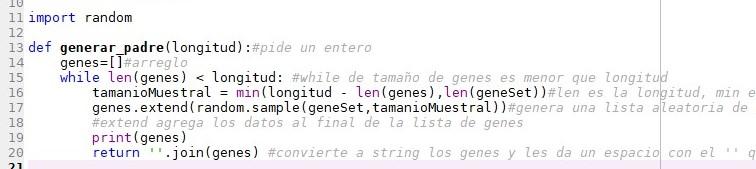
\includegraphics[scale=0.7] {img1.jpg}
\caption{Metodo generarpadre.}
\label{fig:cod1}
\end{figure}

\paragraph{
El segundo m\'etodo llamado $obteneraptitud()$ recibe una variable nino la cual contiene una mutaci\'on , el objetivo de la funci\'on es juntar el objetivo y la conjetura para despu\'es sumarlo en un for, esto se regresa a la funci\'on mostrar para que los datos se muestren en pantalla. Ref: \ref{fig:cod2}
}

\begin{figure}[H]

\includegraphics[scale=0.7] {img2.jpg}
\caption{Metodo obteneraptitud.}
\label{fig:cod2}
\end{figure}

\paragraph{
La siguiente funci\'on llamada mutar() es una de las funciones principales y mas importantes ya que permite hacer variaciones en el gen, esto funciona a partir de crear datos aleatorios y guardarlos en un \'indice. Despu\'es se crea otros valores aleatorios con el rango de los genes para poder cambiar la cadena e intentar mejorar el gen, el resultado se regresa como string y se le da un espacio entre valores. Ref: \ref{fig:cod3}
}
\begin{figure}[H]
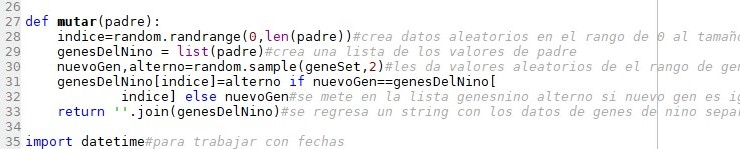
\includegraphics[scale=0.7] {img3.jpg}
\caption{Funci\'on mutar}
\label{fig:cod3}
\end{figure}

\paragraph{ La funci\'on de mostrar() se encarga de mostrar los datos en pantalla de buena manera, obtiene la diferencia de tiempo entre cada gen, muestra tambi\'en la conjetura que en si es la forma en que se va acercando el algoritmo a el objetivo y muestra tambi\'en la aptitud todo eso se muestra en un formato de tres. Ref: \ref{fig:cod4}
}

\begin{figure}[H]
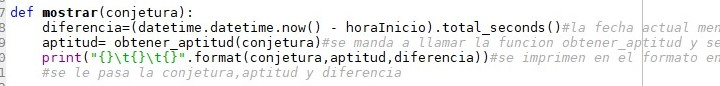
\includegraphics[scale=0.7] {img4.jpg}
\caption{Funci\'on mostrar.}
\label{fig:cod4}
\end{figure}


\paragraph{
Las partes del c\'odigo que no est\'an adentro de una funci\'on son las que normalmente estar\'ian adentro de un main, se encargan de pasar los valores a las funciones y as\'i como se hacen las comparaciones necesarias para saber si el programa debe seguir o terminar e ir agregando la mejor aptitud a un mejor padre. Ref: \ref{fig:cod5}
}

\begin{figure}[H]
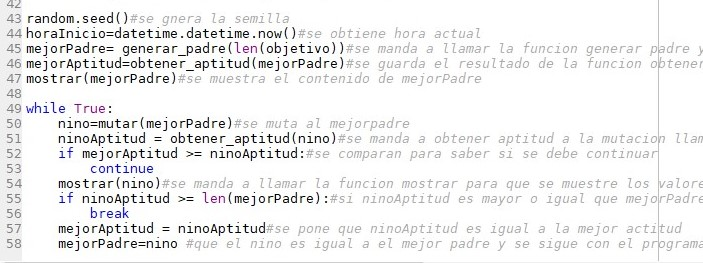
\includegraphics[scale=0.7] {img5.jpg}
\caption{Main.}
\label{fig:cod5}
\end{figure}

\paragraph{
En los resultados se pod\'ia observar lo genial que funciono el algoritmo al lograr encontrar la clave de una manera muy r\'apida. Ref: \ref{fig:cod6}}

\begin{figure}[H]
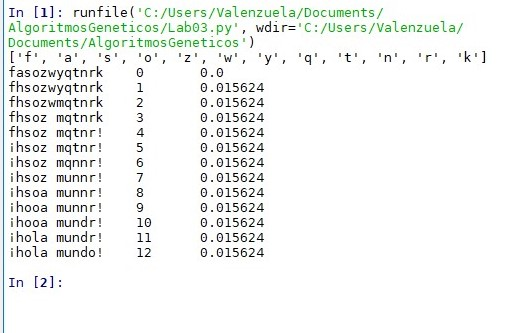
\includegraphics[scale=0.7] {img6.jpg}
\caption{Resultados.}
\label{fig:cod6}
\end{figure}



\section{Conclusi\'on}
\paragraph{Esta practica me mostro el poder de los algoritmos gen\'eticos, tener un algoritmo que puede evolucionar hasta el punto en que d\'e soluci\'on a un problema en especifico hace que tenga miles de aplicaciones, tanto para encontrar claves como en esta pr\'actica, como para mejorar procesos y ayudar a algoritmos a tener una mejor eficiencia.}
\paragraph{
Esta pr\'actica despert\'o a\'un m\'as mi inter\'es en los AG, Y a la vez aprend\'i que Python realmente es muy poderoso, ya que implementar este algoritmo en otro lenguaje como java se volvi\'o bastante complicado en mi caso ya que me encontr\'e con funciones que no existen en java y obligan a hacer mucho m\'as trabajo de c\'odigo que en Python se resume en una l\'inea.}
\paragraph{
Al terminar de comprender todo el c\'odigo logre ver que realmente no hay mucha complejidad en la manera en que trabaja este algoritmo, simplemente se busca mejorar siempre a los hijos y si es necesario se mutan para tener probabilidades de mejorar aun mas y se van escogiendo a los mejores hasta obtener el objetivo. 
}
\section{Referencias}
\paragraph{(2019). Obtenido de sc.ehu.es: www.sc.ehu.es/ccwbayes/docencia/mmcc/docs/temageneticos.pdf}
\paragraph{(2020). Obtenido de w3schools: www.w3schools.com/python/pythondatetime.asp}
\paragraph{(2020). Obtenido de Programiz: www.programiz.com/python-programming/methods/built-in/list}
\paragraph{(2019). Obtenido de Oracle: docs.oracle.com/javase/8/docs/api/java/util/Random.html}
\paragraph{(2017). Obtenido de picodotdev: picodotdev.github.io/blog-bitix/2017/10/obtener-el-minimo-o-maximo-de-dos-una-lista-o-stream-de-valores-en-java/}


\end{document}
